查看本节演示代码：\democode{05}{5.1_Quantum_Neural_Network} \ \democodegithub{05}{5.1_Quantum_Neural_Network}
\subsubsection{背景}
本小节将介绍如何创建量子神经网络，用于解决监督学习中的鸢尾花分类问题；这是经典机器学习中的一个典型任务。

鸢尾花数据集是经典机器学习中常用的数据集。该数据集包含 150 个样本（分为 setosa、versicolor 和 virginica 三类，每类 50 个样本），每个样本具有四个特征：萼片长度、萼片宽度、花瓣长度和花瓣宽度。

我们选取前 100 个样本（setosa 和 versicolor），并从中随机选择 80 个样本作为训练集。随后构建量子神经网络来训练量子分类器（ansatz）。剩余 20 个样本在训练后用于分类测试，目标是尽可能获得最高预测准确率。

首先，将 100 个样本划分为 80 个训练样本和 20 个测试样本。其次，基于训练样本的经典数据计算构建编码器所需的参数。第三，创建编码器，将训练样本的经典数据编码为量子态。第四，设计 ansatz，并使用提出的量子神经网络层和 MindSpore 算子训练其参数，从而得到最终分类器。最后，对剩余 20 个测试样本进行分类，并得到预测准确率。

\subsubsection{数据初始化}
首先，需要导入鸢尾花数据集。

\begin{lstlisting}
from sklearn import datasets

iris_dataset = datasets.load_iris()
\end{lstlisting}

由于只需要选取前 100 个样本，因此执行以下命令。

\begin{lstlisting}
import numpy as np

x = iris_dataset.data[:100, :].astype(np.float32)
x_feature_names = iris_dataset.feature_names
y = iris_dataset.target[:100].astype(int)
y_target_names = iris_dataset.target_names[:2]
\end{lstlisting}

为了更直观地理解由这 100 个样本组成的数据集，可以执行以下命令，绘制所有样本不同特征之间组合关系的散点图。

\begin{lstlisting}
import matplotlib.pyplot as plt

feature_name = {0: 'sepal length', 1: 'sepal width', 2: 'petal length', 3: 'petal width'}
axes = plt.figure(figsize=(23, 23)).subplots(4, 4)

colormap = {0: 'r', 1: 'g'}
cvalue = [colormap[i] for i in y]

for i in range(4):
    for j in range(4):
        if i != j:
            ax = axes[i][j]
            ax.scatter(x[:, i], x[:, j], c=cvalue)
            ax.set_xlabel(feature_name[i], fontsize=22)
            ax.set_ylabel(feature_name[j], fontsize=22)

plt.show()
\end{lstlisting}

%\begin{figure*}[t]
%\centering
%\label{irisdatasetfigure}
%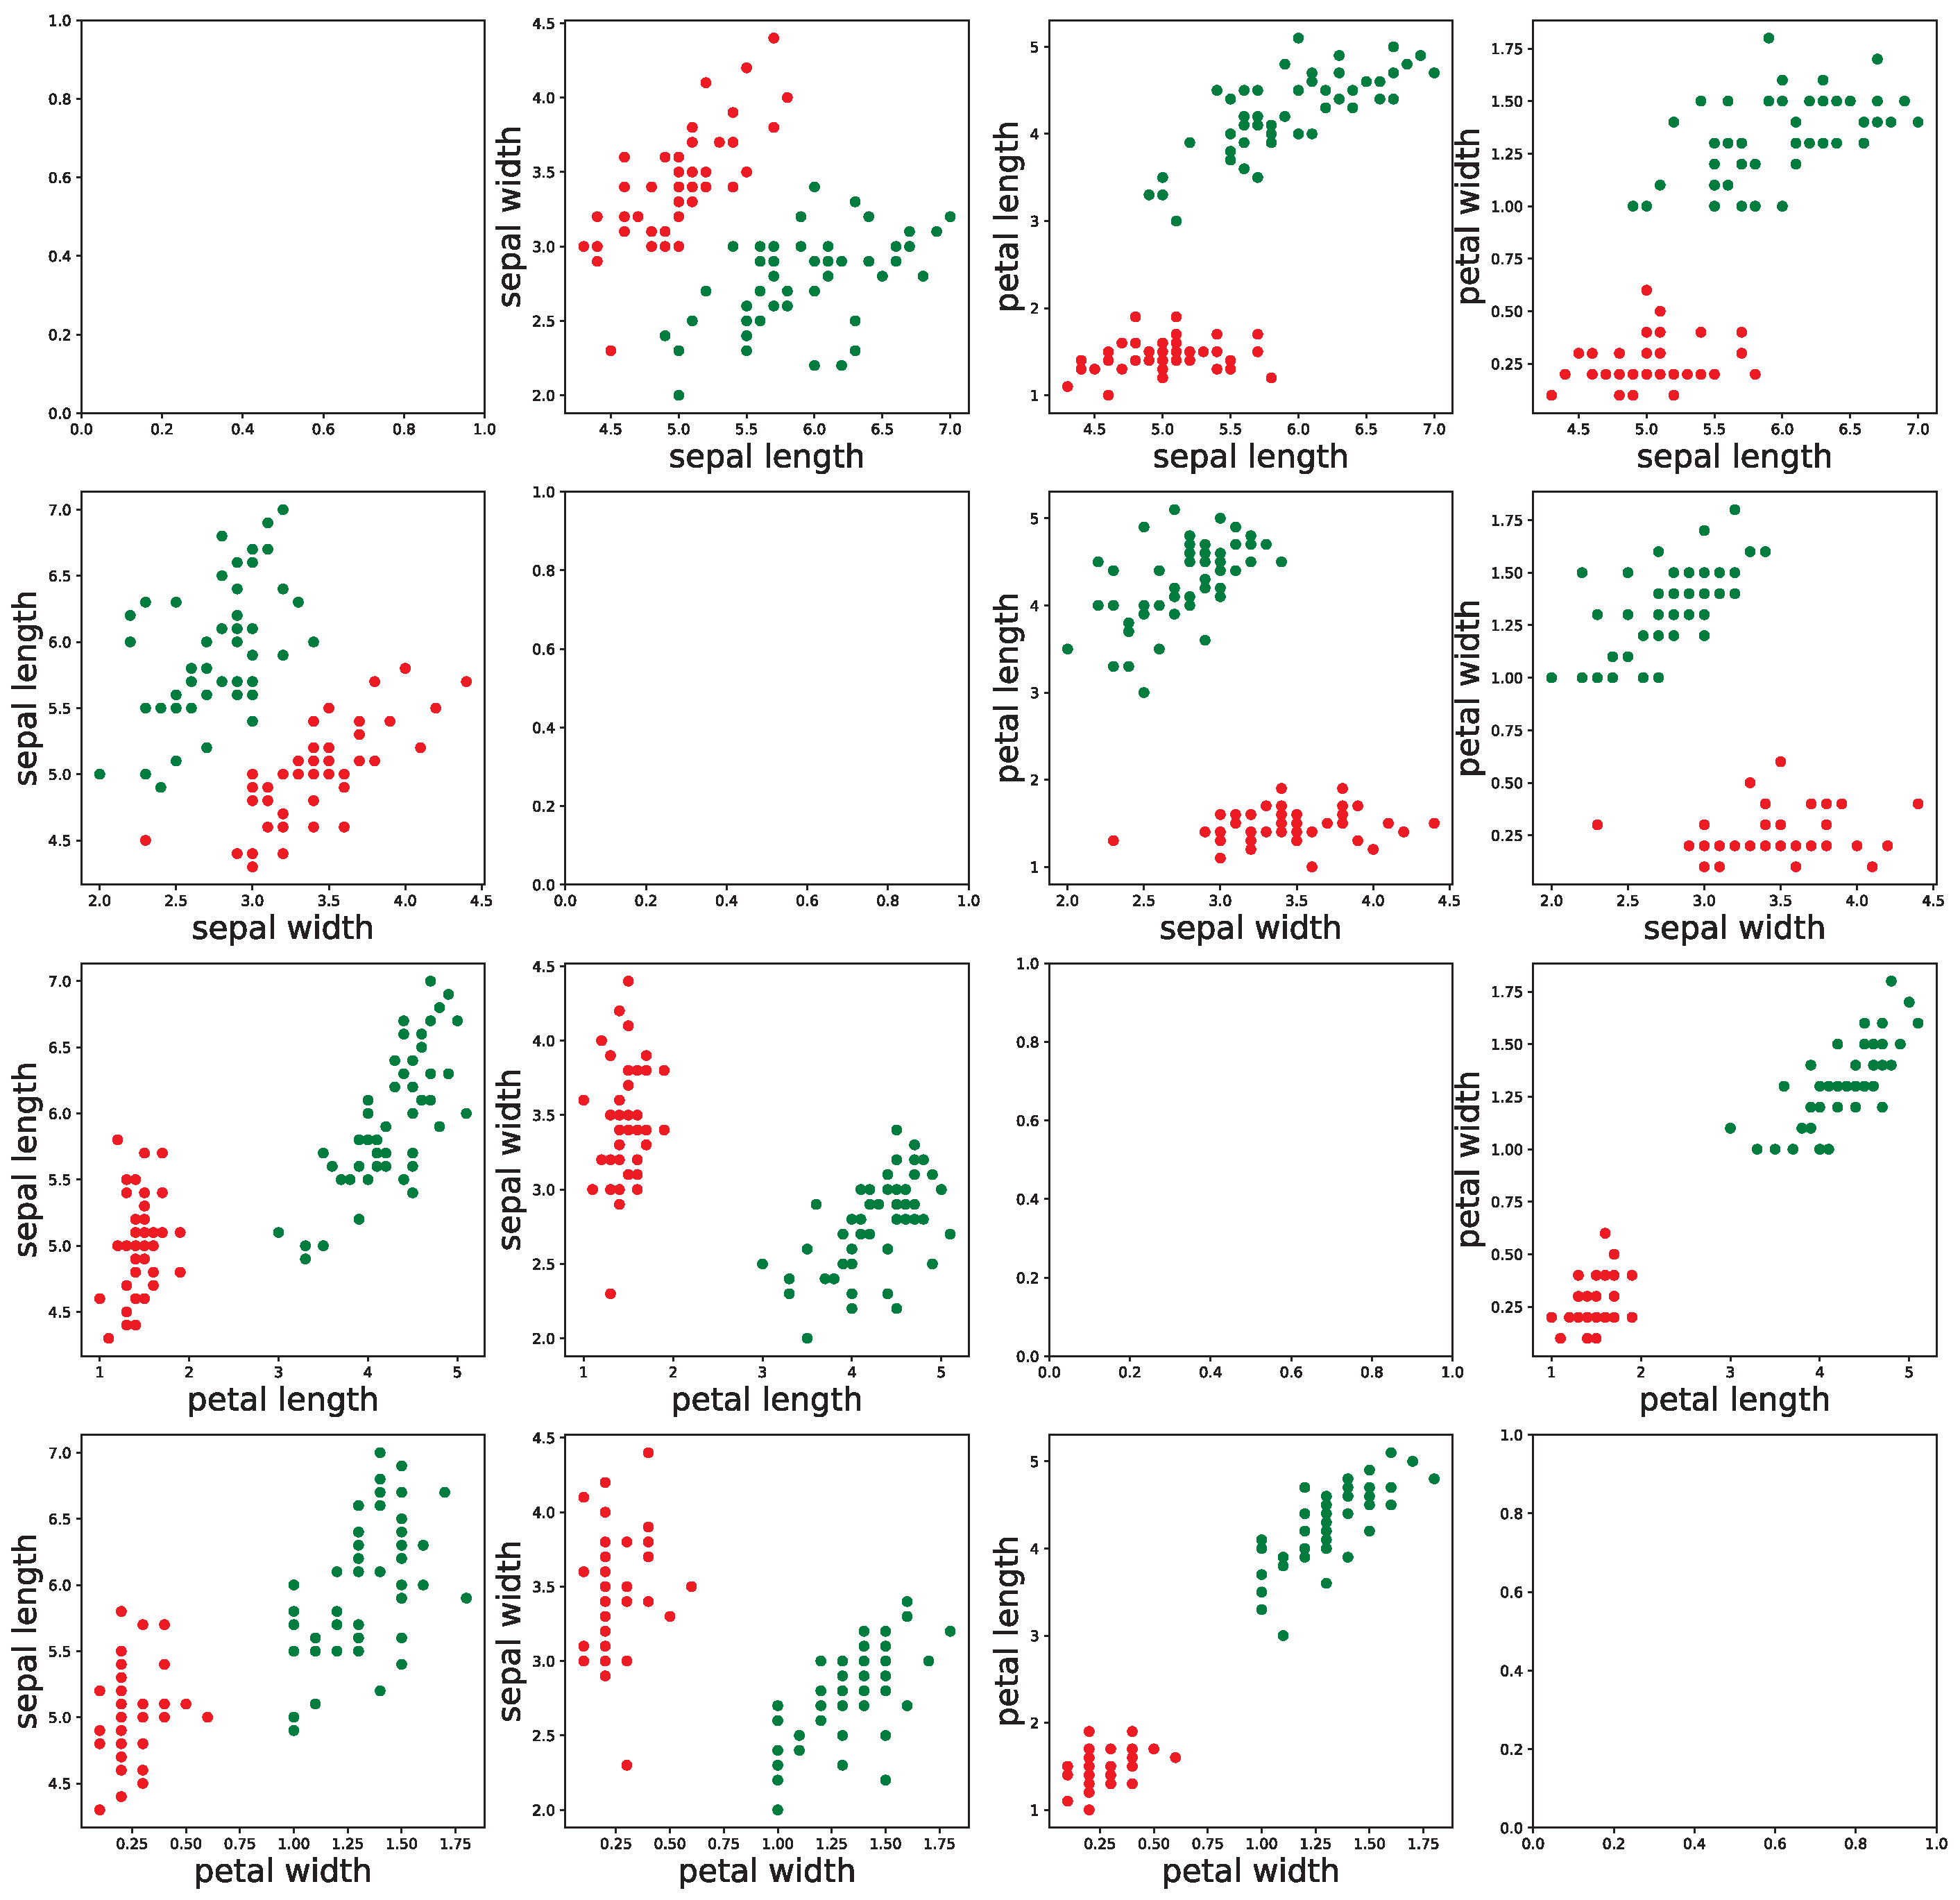
\includegraphics[width=0.8\textwidth]{5.1_figures/irisdataset_figure.eps}
%\caption{Visualization of iris dataset}
%\end{figure*}

%As seen in the images above, the red dots indicate samples with the label ``0'', while the green dots represent samples with the label ``1''.

\subsubsection{编码器与 Ansatz}
接下来，计算构建编码器所需的参数。执行以下命令。

\begin{lstlisting}
alpha = x[:, :3] * x[:, 1:]
x = np.append(x, alpha, axis=1)
\end{lstlisting}

构造特征是数据预处理中常用的技术。因此，此时每个样本具有 7 个特征：前四个特征值为原始特征值，后三个特征值由上述预处理计算得到。具体计算公式如下：

\begin{eqnarray}\label{5.1dataprocessing}
    X_{i+4}^{j} = X_{i}^{j} * X_{i+1}^{j},
\end{eqnarray}
其中 $i = 0, 1, 2$，$j = 1, 2, \cdots, 100$。

最后，通过运行下面的命令，将当前数据集划分为训练集和测试集。

\begin{lstlisting}
from sklearn.model_selection import train_test_split

x_train, x_test, y_train, y_test = train_test_split(x, y, test_size=0.2, random_state=0, shuffle=True)
\end{lstlisting}

此时训练集中有 80 个样本，测试集中有 20 个样本，每个样本都有 7 个特征。

接下来，需要在 MindSpore Quantum 中构建编码器，将经典数据编码为量子态。

这里采用的编码方法是 IQP 编码（Instantaneous Quantum Polynomial encoding）。一般而言，编码器的构建方式并非固定不变；可以根据当前问题的需求使用多种编码技术，有时还可以修改编码器以提升性能。

编码器中参数 $\alpha_0$, $\alpha_1$, $\cdots$,$\alpha_6$ 的取值由式~\eqref{5.1dataprocessing} 数据处理中得到的 7 个特征值代入。

现在，可以通过以下代码在 \MindQuantum\ 中构建编码器量子线路（见图~\ref{5.1encoder-circuit}）。

\begin{lstlisting}
from mindquantum import *

encoder = Circuit()

encoder += UN(H, 4)
for i in range(4):
    encoder += RZ(f'alpha{i}').on(i)
for j in range(3):
    encoder += X.on(j+1, j)
    encoder += RZ(f'alpha{j+4}').on(j+1)
    encoder += X.on(j+1, j)

encoder = encoder.no_grad()
encoder.svg()
\end{lstlisting}

\begin{figure}[H]
    \centering
    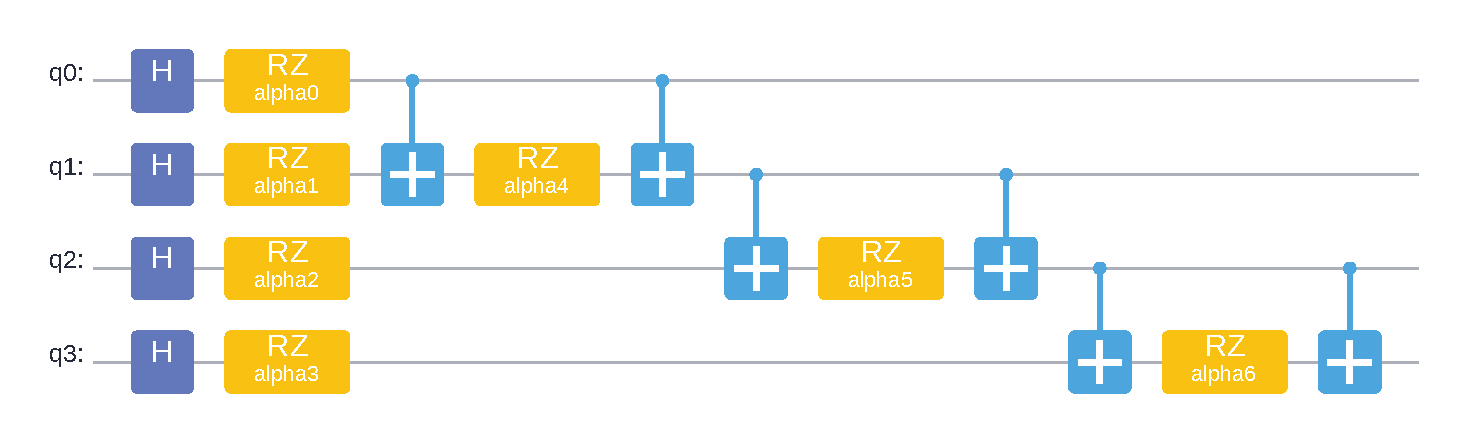
\includegraphics[width=0.49\textwidth]{5.1_figures/encoder-circuit.eps}
    \caption{IQP 编码器}
    \label{5.1encoder-circuit}
\end{figure}

从编码器线路可以看出，该量子线路由 17 个量子门组成，其中 7 个为参数化量子门，参数分别为 $\alpha_0$, $\alpha_1$, $\cdots$,$\alpha_6$。编码器线路调控的量子比特数量为 4。

此外，还需要在 MindSpore Quantum 中构建 ansatz。

与编码器类似，ansatz 的构建策略也很灵活，可以用于考察不同策略的有效性。

在本例中，我们使用 \HardwareEfficientAnsatz。通过以下代码得到的量子线路如图~\ref{5.1ansatz-circuit} 所示。

\begin{lstlisting}
ansatz = HardwareEfficientAnsatz(4, single_rot_gate_seq=[RY], entangle_gate=X, depth=3).circuit
ansatz.svg()
\end{lstlisting}

\begin{figure}[H]
    \centering
    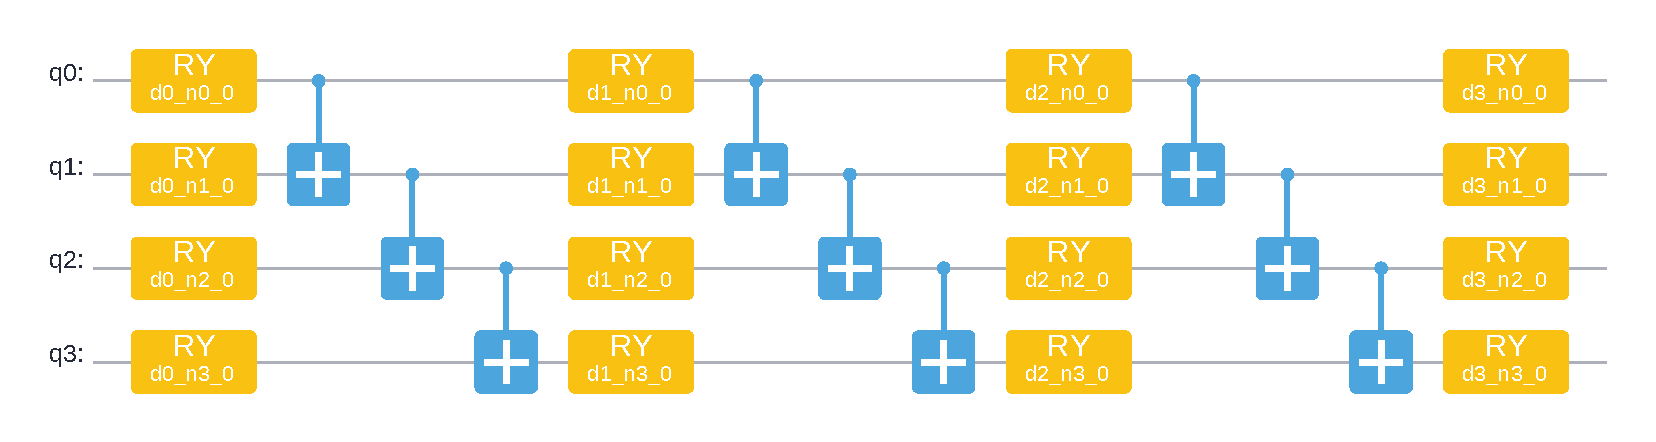
\includegraphics[width=0.49\textwidth]{5.1_figures/ansatz-circuit.eps}
    \caption{硬件高效 Ansatz}
    \label{5.1ansatz-circuit}
\end{figure}

从 ansatz 线路可以看出，该量子线路由 25 个量子门组成，其中 16 个为参数化量子门，参数分别为 $d0\_n0\_0$, $d0\_n1\_0$, $d0\_n2\_0$, $\cdots$。ansatz 线路调控的量子比特数量为 4。

在这种情况下，可以通过以下代码将编码器和 ansatz 组合成完整量子线路（见图~\ref{5.1total-circuit}）。

\begin{lstlisting}
circuit = encoder.as_encoder() + ansatz.as_ansatz()
circuit.svg()
\end{lstlisting}

\begin{figure}[H]
    \centering
    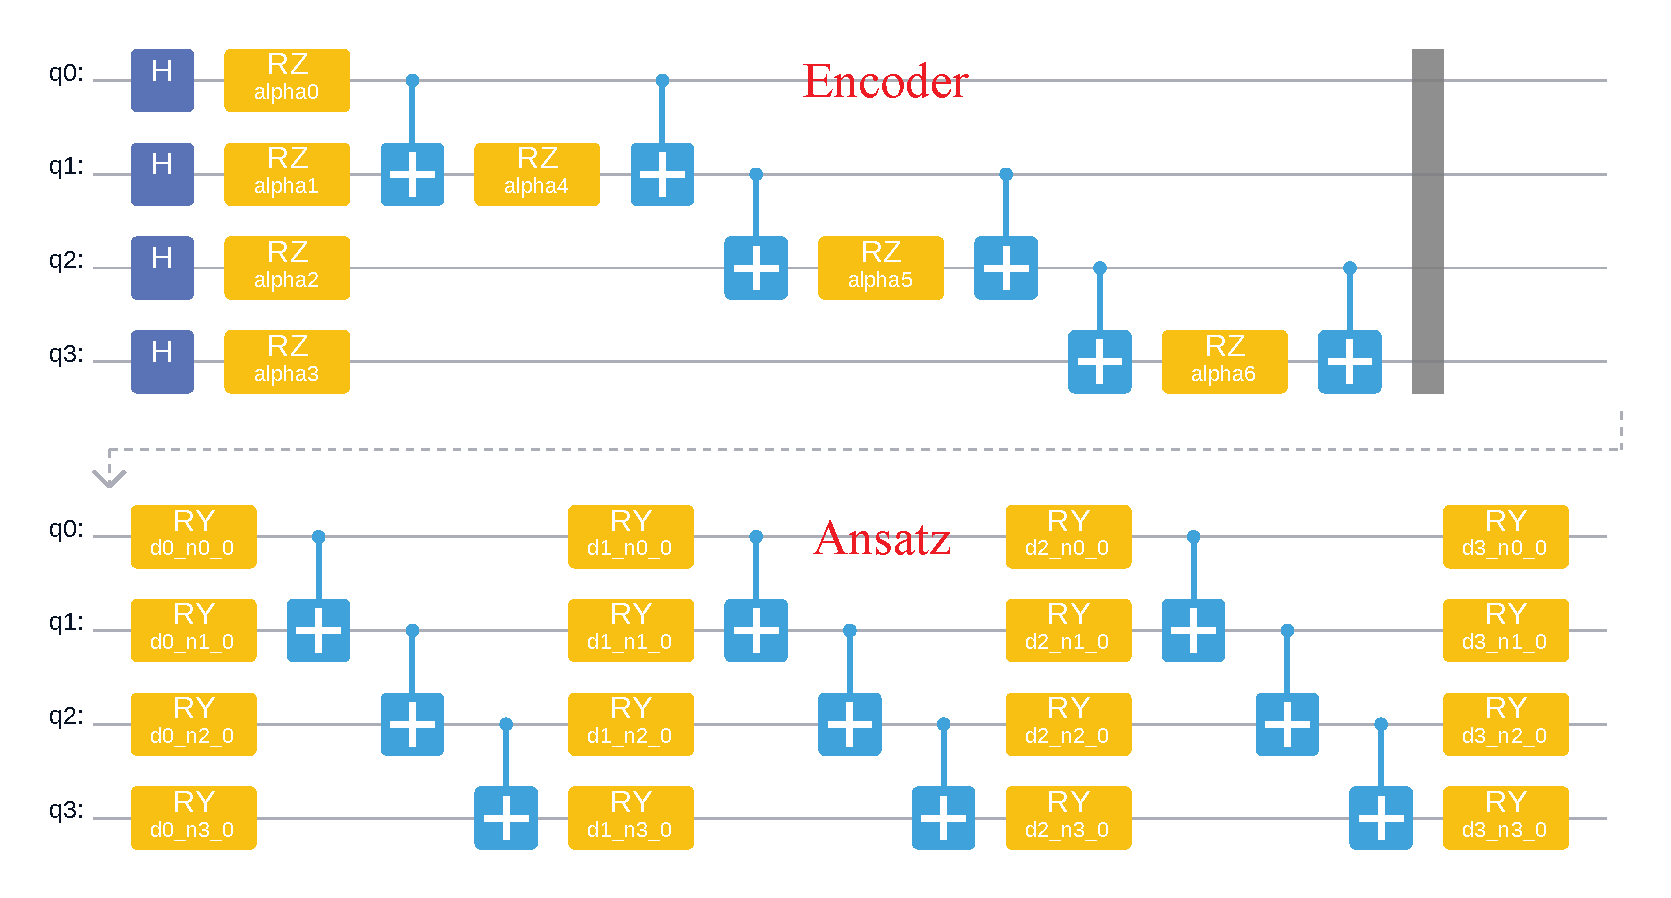
\includegraphics[width=0.49\textwidth]{5.1_figures/total-circuit.eps}
    \caption{完整量子线路}
    \label{5.1total-circuit}
\end{figure}

\subsubsection{哈密顿量}
我们分别在第二个和第三个量子比特上执行 Pauli $Z$ 算符测量，以创建对应的哈密顿量。执行以下代码。

\begin{lstlisting}
hams = [Hamiltonian(QubitOperator(f'Z{i}')) for i in [2, 3]]
for h in hams:
    print(h)
\end{lstlisting}

\begin{lstlisting}
1 [Z2]
1 [Z3]
\end{lstlisting}

从上述打印结果可以看出，此时构建了两个哈密顿量，分别是在第二个和第三个量子比特上作用 Pauli $Z$ 算符，并将系数设为 1。通过 Pauli $Z$ 算符测量，我们将得到两个哈密顿量测量值。

如果第一个测量值较大，则样本会被分类为标签为 ``0'' 的类别。类似地，如果第二个测量值较大，则样本会被分类为标签为 ``1'' 的类别。通过训练量子神经网络，我们期望训练样本中标签为 ``0'' 的样本具有更大的第一个测量值，标签为 ``1'' 的样本具有更大的第二个测量值。最后，将训练好的模型用于预测新样本的类别。

\subsubsection{训练}
通过以下命令构建量子神经网络。

\begin{lstlisting}
import mindspore as ms
from mindquantum.framework import MQLayer
from mindquantum.simulator import Simulator

ms.set_context(mode=ms.PYNATIVE_MODE, device_target="CPU")
ms.set_seed(1)
sim = Simulator('mqvector', circuit.n_qubits)
grad_ops = sim.get_expectation_with_grad(hams,
                                         circuit,
                                         parallel_worker=5)
QuantumNet = MQLayer(grad_ops)
QuantumNet
\end{lstlisting}

\begin{lstlisting}
MQLayer<
  (evolution): MQOps<4 qubits mqvector VQA Operator>
  >
\end{lstlisting}

从上述打印结果可以看出，我们已经成功构建了一个量子机器学习层，它可以与 MindSpore 中的其他算子无缝组成更大的机器学习网络。

接下来，需要定义损失函数并设置待优化参数。随后，将构建好的量子机器学习层与 MindSpore 算子组合成更大的机器学习网络。最后，对模型进行训练。%Follow the command below.

\begin{lstlisting}
from mindspore import LossMonitor, Model
from mindspore.nn import SoftmaxCrossEntropyWithLogits, Adam, Accuracy
from mindspore.dataset import NumpySlicesDataset
from mindspore.train import Callback

loss = SoftmaxCrossEntropyWithLogits(sparse=True, reduction='mean')
opti = Adam(QuantumNet.trainable_params(), learning_rate=0.1)

model = Model(QuantumNet, loss, opti, metrics={'Acc': Accuracy()})

train_loader = NumpySlicesDataset({'features': x_train, 'labels': y_train}, shuffle=False).batch(5)
test_loader = NumpySlicesDataset({'features': x_test, 'labels': y_test}).batch(5)

class StepAcc(ms.Callback):
    def __init__(self, model, test_loader):
        self.model = model
        self.test_loader = test_loader
        self.acc = []

    def step_end(self, run_context):
        self.acc.append(self.model.eval(self.test_loader, dataset_sink_mode=False)['Acc'])

monitor = LossMonitor(16)

acc = StepAcc(model, test_loader)

model.train(20, train_loader, callbacks=[monitor, acc], dataset_sink_mode=False)
\end{lstlisting}

\begin{lstlisting}
epoch: 1 step: 16, loss is 0.6140301823616028
epoch: 2 step: 16, loss is 0.48262983560562134
epoch: 3 step: 16, loss is 0.43457236886024475
epoch: 4 step: 16, loss is 0.4101267457008362
epoch: 5 step: 16, loss is 0.4027639925479889
epoch: 6 step: 16, loss is 0.39859312772750854
epoch: 7 step: 16, loss is 0.39496558904647827
epoch: 8 step: 16, loss is 0.3970319926738739
epoch: 9 step: 16, loss is 0.3954522907733917
epoch: 10 step: 16, loss is 0.39520972967147827
epoch: 11 step: 16, loss is 0.3955090641975403
epoch: 12 step: 16, loss is 0.3953099250793457
epoch: 13 step: 16, loss is 0.39525243639945984
epoch: 14 step: 16, loss is 0.3952508568763733
epoch: 15 step: 16, loss is 0.39521533250808716
epoch: 16 step: 16, loss is 0.39519912004470825
epoch: 17 step: 16, loss is 0.39518338441848755
epoch: 18 step: 16, loss is 0.395169198513031
epoch: 19 step: 16, loss is 0.39515653252601624
epoch: 20 step: 16, loss is 0.3951443135738373
\end{lstlisting}

训练过程中损失值持续下降，并在约 20 次迭代后趋于稳定，最终收敛在约 0.395。

根据上述收敛情况，可以展示训练过程中模型预测准确率的变化。%Run the following code.

\begin{lstlisting}
plt.plot(acc.acc)
plt.title('Statistics of accuracy', fontsize=20)
plt.xlabel('Steps', fontsize=20)
plt.ylabel('Accuracy', fontsize=20)

plt.show()
\end{lstlisting}

\begin{figure}[H]
    \centering
    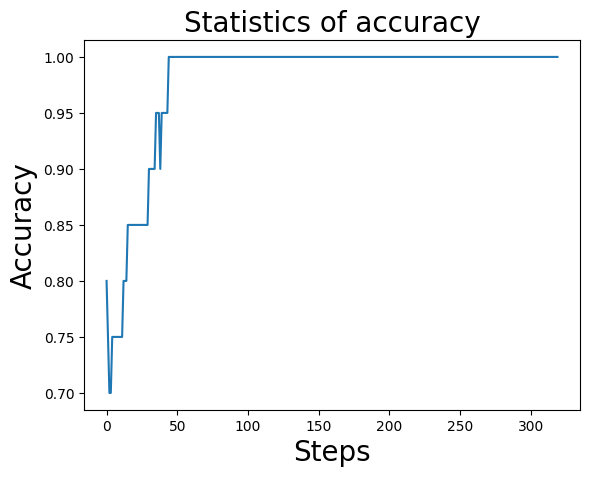
\includegraphics[width=0.4\textwidth]{5.1_figures/Statistics_of_accuracy.png}
    \caption{准确率统计}
    \label{5.1Statistics_of_accuracy}
\end{figure}

从图~\ref{5.1Statistics_of_accuracy} 可以看出，预测准确率在约 50 步后收敛到 1.00。

\subsubsection{预测}
最后，将训练好的模型应用到测试集上。
\begin{lstlisting}
from mindspore import ops

predict = np.argmax(ops.Softmax()(model.predict(ms.Tensor(x_test))), axis=1)
correct = model.eval(test_loader, dataset_sink_mode=False)

print("Predicted classification result:", predict)
print("Actual classification result:", y_test)

print(correct)
\end{lstlisting}

\begin{lstlisting}
Predicted classification result: [0 1 0 1 1 1 0 1 1 1 1 1 1 0 0 0 0 0 0 0]
Actual classification result: [0 1 0 1 1 1 0 1 1 1 1 1 1 0 0 0 0 0 0 0]
{'Acc': 1.0}
\end{lstlisting}

从上述打印结果可以看出，模型预测准确率达到 $100\%$，这意味着预测分类结果与实际分类结果完全一致。
